\documentclass[11pt]{beamer}
\usetheme{Antibes}
\usepackage[utf8]{inputenc}
\usepackage{amsmath}
\usepackage{amsfonts}
\usepackage{amssymb}
\usepackage{amsthm}
\usepackage{graphicx}
\author{Paul LANDRIER \\ Supervised by Silviu Maniu}
\title{Adaptation of Semiring Provenance}

\usepackage{subcaption}
\usepackage{tikz}
\newcommand{\binset}{\{0,1\}}

\newcommand{\utup}{\text{$U$-\textbf{Tup}}}
\newcommand{\vtup}[1]{\text{$#1$-\textbf{Tup}}}

\newcommand{\bb}[1]{\mathbb{#1}}

%\setbeamercovered{transparent} 
%\setbeamertemplate{navigation symbols}{} 
%\logo{} 
%\institute{LIG} %ENS ? UGA ?
\date{} 
%\subject{}

\begin{document}

\begin{frame}
\titlepage
\end{frame}

\begin{frame}
\tableofcontents
\end{frame}

\AtBeginSection[]{
  \begin{frame}
  \vfill
  \centering
  \begin{beamercolorbox}[sep=8pt,center,shadow=true,rounded=true]{title}
    \usebeamerfont{title}\insertsectionhead\par%
  \end{beamercolorbox}
  \vfill
  \end{frame}
}

\section{Existing framework - Provenance in databases}
\subsection{Example}
%And in graphs ?
\begin{frame}{Situation}

This whole section is entirely based on \cite{green_provenance_2007}.

	\begin{figure}
	\begin{subfigure}{0.45\textwidth}
        \centering
        $\begin{array}{| c  c  c |}
            \hline
            ClientName & \textit{Country} & Product \\
            (A) & (B) & (C) \\
            \hline 
            \hline
            Alice & USA & tea \\
            \hline
            Bob & USA & coffee \\
            \hline
            Charlie & FR & coffee \\
            \hline
        \end{array}$
      \end{subfigure}
      \begin{subfigure}{0.45\textwidth}
        \centering
        $\begin{array}{| c  c  |}
            \hline
            A & C \\
            \hline 
            \hline
            Alice & tea \\
            \hline
            Alice & coffee  \\
            \hline
            Bob & tea  \\
            \hline
            Bob & coffee  \\
            \hline
            Charlie & coffee  \\
            \hline
        \end{array}$
        \label{fig:calc_bag}
    	\end{subfigure}
        \caption{Databases $D$ and $q(D)$.}
        \label{fig:base_database}
	\end{figure}
	
	$$ q(R) \overset{\mathrm{def}}{=} \pi_{AC}(\pi_{AB} R \Join \pi_{BC} R \cup \pi_{AC} R \Join \pi_{BC} R)$$

\end{frame}

\begin{frame}{Situation}

\begin{figure}
\begin{subfigure}{0.45\textwidth}
$\begin{array}{| c  c  c |  c |}
            \hline
            A & B & C &  \\
            \hline 
            \hline
            Alice & USA & tea & 2 \\
            \hline
            Bob & USA & coffee & 5 \\
            \hline
            Charlie & FR & coffee & 1 \\
            \hline
        \end{array}$
\end{subfigure}
\begin{subfigure}{0.45\textwidth}
$\begin{array}{| c  c  c |  c |}
            \hline
            A & B & C &  \\
            \hline 
            \hline
            Alice & USA & tea & b_1 \\
            \hline
            Bob & USA & coffee & b_2 \\
            \hline
            Charlie & FR & coffee & b_3 \\
            \hline
        \end{array}$
\end{subfigure}
\end{figure}

\begin{tiny}

\begin{figure}
\centering
\begin{subfigure}{0.5\textwidth}
$\begin{array}{| c  c  | c |}
            \hline
            A & C & \\
            \hline 
            \hline
            Alice & \textit{tea} & 2 \cdot 2 + 2 \cdot 2 = 8\\
            \hline
            Alice & \textit{coffee} & 2 \cdot 5 = 10 \\
            \hline
            Bob & \textit{tea} & 2 \cdot 5 = 10 \\
            \hline
            Bob & \textit{coffee} & 5 \cdot 5 + 5 \cdot 5 + 5 \cdot 1 = 55 \\
            \hline
            Charlie & \textit{coffee} & 1 \cdot 1 + 1 \cdot 1 + 5 \cdot 1 = 7 \\
            \hline
           \end{array}$
\end{subfigure}
\begin{subfigure}{0.5\textwidth}
$\begin{array}{| c  c  | c |}
            \hline
            A & C & \\
            \hline 
            \hline
            Alice & \textit{tea} & (b_1 \wedge b_1) \vee (b_1 \wedge b_1) = b_1\\
            \hline
            Alice & \textit{coffee} & b_1 \wedge b_2 \\
            \hline
            Bob & \textit{tea} & b_1 \wedge b_2 \\
            \hline
            Bob & \textit{coffee} & (b_2 \wedge b_2) \vee (b_2 \wedge b_2) \vee (b_2 \wedge b_1)  \\
            \hline
            Charlie & \textit{coffee} & (b_3 \wedge b_3) \vee (b_3 \wedge b_3) \vee (b_2 \wedge b_3) \\
            \hline
           \end{array}$
\end{subfigure}
\end{figure}
\end{tiny}
\end{frame}

\subsection{Semirings and polynomials for provenance}
\begin{frame}{Polynomials for provenance}

We abstract the two preceeding computations with variables $p,r,s$ and abstract operations $+$ and $\cdot$.

\begin{figure}
$\begin{array}{| c  c  c |  c |}
            \hline
            A & B & C &  \\
            \hline 
            \hline
            Alice & USA & \textit{tea} & p \\
            \hline
            Bob & USA & \textit{coffee} & r \\
            \hline
            Charlie & FR & \textit{coffee} & s \\
            \hline
        \end{array}$

\end{figure}

\begin{figure}
$\begin{array}{| c  c  | c |}
            \hline
            A & C & \\
            \hline 
            \hline
            Alice & \textit{tea} & 2p^2 \\
            \hline
            Alice & \textit{coffee} & pr \\
            \hline
            Bob & \textit{tea} & pr \\
            \hline
            Bob & \textit{coffee} & 2r^2 + rs\\
            \hline
            Charlie & \textit{coffee} & 2s^2 + rs \\
            \hline
           \end{array}$
\end{figure}

\end{frame}

\begin{frame}[allowframebreaks]{Positive Relational Algebra on $K$-relations}

\begin{list}{}{}
		
			\item[\textbf{empty relation}] There is $\emptyset : \left\lbrace 
			\begin{array}{c c c}
			\utup & \to & K \\
			t & \mapsto & 0_K
			\end{array}
			  \right.$.
		
			\item[\textbf{union}] Let $R_1,R_2 : \utup \to K$ be two $K$-relations.
			
			Then we define $R_1 \cup R_2 : 
			\left\lbrace 
			\begin{array}{c c c}
			\text{$U$-\textbf{Tup}} & \to & K \\
			t & \mapsto & R_1(t) + R_2(t)
			\end{array}
			  \right.$.
			  
			 \item[\textbf{projection}] Let $R : \utup \to K$ be a $K$-relation and let $V \subseteq U$ be a subdomain of $U$.
			 
			Then we define $\pi_VR: 
			\left\lbrace 
			\begin{array}{c c c}
			\text{$U$-\textbf{Tup}} & \to & K \\
			t & \mapsto & \underset{t' \in supp(R) \text{ and } t'_{|V}=t}{\sum} R(t')
			\end{array}
			  \right.$.
			  
			 Where $t'_{|V} \in \text{$V$-\textbf{Tup}}$ is the restriction of $t' \in \utup$ seen as a function $U \to \bb{D}$ to the subset $V$. Since $supp(R)$ is finite, the sum is finite.
		
			\item[\textbf{selection}] Let $R : \utup \to K$ be a $K$-relation and $\textbf{P} : \utup \to \{0_K,1_K\}$ be a predicate.
			
			Then we define $\sigma_{\textbf{P}} R: 
			\left\lbrace 
			\begin{array}{c c c}
			\text{$U$-\textbf{Tup}} & \to & K \\
			t & \mapsto & R(t) \cdot \textbf{P}(t)
			\end{array}
			  \right.$.
			  
			 \item In the two remaining definitions, be aware that the set of attributes over which functions are defined changes. 
			  
			\item[\textbf{natural join}] Let $U_1,U_2$ be two finite sets of attributes. Let $R_1 : \vtup{U_1} \to K$ and $R_2 : \vtup{U_2} \to K$ be two $K$ relations.
			
		Then we define $R_1 \Join R_2: 
			\left\lbrace 
			\begin{array}{c c c}
			\vtup{(U_1 \cup U_2)} & \to & K \\
			t & \mapsto & R_1(t_{|U_1}) \cdot R_2(t_{|U_2})
			\end{array}
			  \right.$.
			  
			  
			 \item[\textbf{renaming}] Let $R : \utup \to K$ be a $K$-relation and $\beta : U \to U'$ be a bijection.
			 
			 Then we define $\rho_\beta R: 
			\left\lbrace 
			\begin{array}{c c c}
			\vtup{U'} & \to & K \\
			t & \mapsto & R(t \circ \beta)
			\end{array}
			  \right.$.
		
		\end{list}

\end{frame}

\begin{frame}{Semirings for provenance}

A very nice property :

\begin{block}{Semirings are a good choice for provenance}
The $\mathcal{RA}^+$ equalities:
		
		\begin{itemize}
		
			\item Union is associative, commutative and has identity $\emptyset$;
			
			\item Join is associative, commutative and distributive over union;
			
			\item Projections and selections commute with each other as well as with unions and joins;
			
			\item For all $R$, $\sigma_{\textbf{false}}(R)=\emptyset$ and $\sigma_{\textbf{true}}(R)=R$
			
		\end{itemize}
		
		are satisfied if and only if $(K,+,\cdot,0_K,1_K)$ is a commutative semiring.
\end{block}

\end{frame}

\section{Provenance for computation graphs}
\subsection{Computation Graphs}

\begin{frame}{Definition}

\begin{block}{Definition - Computation Graph}
A computation graph $(V,E,Fun,Op,F,Operator)$ over a set $S$ is a directed acyclic graph $(V,E)$ together with:

\begin{itemize}

	\item two subsets $F \subset (S \to S)$ and $Operator \subset (S^{(\bb{N})} \to S)$,

	\item a function $Fun : E \to F$,
	
	\item a function $Op : V \to Operator$.
		
\end{itemize}
\end{block}

\end{frame}

\begin{frame}{An Example} % And link with NN

	Goal : derive a computation for the function $f(x)=e^{x^2}(x^2 + 2x + 2)$ using only the linear, square, "plus constant" and exponential functions, with $+$ and $\times$ operators.

	\begin{figure}[!h]
	\centering
	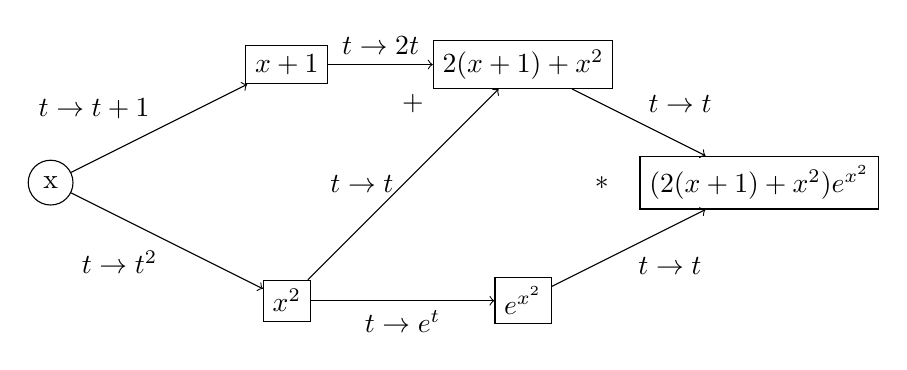
\begin{tikzpicture}
	
		\node[circle,draw] (x) at (0,0) {x};
		\node[rectangle,draw] (a) at (3,1.5) {$x+1$};
		\node[rectangle,draw] (b) at (3,-1.5) {$x^2$};
		\node[rectangle,draw] (c) at (6,1.5) {$2(x+1) + x^2$};
		\node at (4.6,1) {$+$};
		\node[rectangle,draw] (d) at (6,-1.5) {$e^{x^2}$};
		\node[rectangle,draw] (e) at (9,0) {$(2(x+1) + x^2)e^{x^2}$};
		\node at (7,0) {$*$};
		
		\path[->] (x) edge node[midway,above left] 
			{$t \to t+1$} (a);
		\path[->] (x) edge node[midway,below left]
			{$t \to t^2$} (b);
		\path[->] (a) edge node[midway,above] 
			{$t \to 2t$} (c);
			
		\path[->] (b) edge node[midway,left] 
			{$t \to t$} (c);
		\path[->] (b) edge node[midway,below] 
			{$t \to e^t$} (d);
		\path[->] (c) edge node[midway,above right]
			{$t \to t$} (e);
		\path[->] (d) edge node[midway,below right] 
			{$t \to t$} (e);
		
	\end{tikzpicture}
	\caption{One possible computation graph of $f$.}
	\label{fig:graphe_calc_ex}
	\end{figure}

\end{frame}

\begin{frame}{Links with Neural Networks}

\begin{block}{Property}
A Deep Neural Network can be represented by a computation graph. 
\end{block}

\begin{figure}[!h]
\small
\label{fig:graph_calc_execution}
\centering
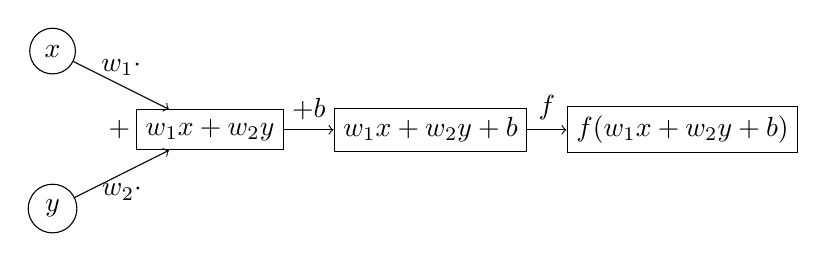
\begin{tikzpicture}

	\def\layersep{2cm}	
	
	\node[circle,draw] (x) at (0,1) {$x$};
	\node[circle,draw] (y) at (0,-1) {$y$};
	\node[rectangle,draw] (a) at (\layersep,0) {$w_1 x + w_2 y$};
	\node (plus) at (\layersep - 1.15cm,0) {+};
	\node[rectangle,draw] (c) at (2.4*\layersep,0) {$w_1 x + w_2 y + b$};
	\node[rectangle,draw] (e) at (4*\layersep,0) {$f(w_1 x + w_2 y + b)$};
	
	\path[->] (x) edge node[midway,above] {$w_1 \cdot $} (a);
	\path[->] (y) edge node[midway, below] {$w_2 \cdot$} (a);
	
	\path[->] (a) edge node[midway,above] {$ + b$} (c);
	
	\path[->] (c) edge node[midway,above] {$f$} (e);
	
	
\end{tikzpicture}
\caption{Computation graph of a perceptron.}
\end{figure}
\end{frame}

\subsection{Abstraction of Computation Graphs}
\begin{frame}{Abstract Computation Graph}

\begin{block}{Definition - Computation Graph over a Set}
A computation graph $(V,E,Fun,Op,F,Operator)$ over a set $S$ is a directed acyclic graph $(V,E)$ together with :

\begin{itemize}

	\item two subsets $F \subset (S \to S)$ and $Operator \subset (S^{(\bb{N})} \to S)$,

	\item a function $Fun : E \to F$,
	
	\item a function $Op : V \to Operator$.
		
\end{itemize}
\end{block}

\begin{block}{Definition - Computation Graph over a General Algebraic Structure}
A generalised computation graph $(V,E,Fun,F)$ is a directed acyclic graph $(V,E)$ together with :

\begin{itemize}

	\item an algebraic structure $(F,+,\circ,0_F,id)$,

	\item a function $Fun : E \to F$.
		
\end{itemize}
\end{block}

\end{frame}

\begin{frame}{Interpretation of a Generalized Computation Graph}

\begin{figure}[!h]
	\centering
	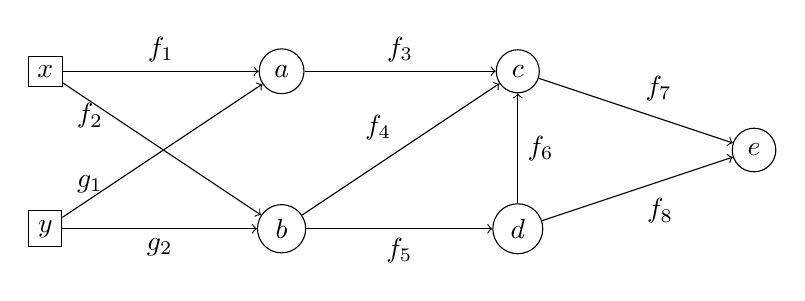
\begin{tikzpicture}
	
		\node[rectangle,draw] (x) at (0,1) {$x$};
		\node[rectangle,draw] (y) at (0,-1) {$y$};
		\node[circle,draw] (a) at (3,1) {$a$};
		\node[circle,draw] (b) at (3,-1) {$b$};
		\node[circle,draw] (c) at (6,1) {$c$};
		\node[circle,draw] (d) at (6,-1) {$d$};
		\node[circle,draw] (e) at (9,0) {$e$};
		
		\path[->] (x) edge node[midway,above] 
			{$f_1$} (a);
		\path[->] (x) edge node[near start, left=0cm]
			{$f_2$} (b);
		\path[->] (y) edge node[near start, left=0cm] 
			{$g_1$} (a);
		\path[->] (y) edge node[midway,below]
			{$g_2$} (b);
		\path[->] (a) edge node[midway,above] 
			{$f_3$} (c);
			
		\path[->] (b) edge node[midway,above left] 
			{$f_4$} (c);
		\path[->] (b) edge node[midway,below] 
			{$f_5$} (d);
		\path[->] (d) edge node [midway,right] 
			{$f_6$}(c);
		\path[->] (c) edge node[midway,above right]
			{$f_7$} (e);
		\path[->] (d) edge node[midway,below right] 
			{$f_8$} (e);
	\end{tikzpicture}
	\caption{An abstract computation graph.}
	\label{fig:graphe_calc_abstr}
\end{figure}
The expression represented by the figure above is $f_7 \circ [f_3 \circ (f_1 \circ x + g_1 \circ y) + f_4 \circ ( f_2 \circ x + g_2 \circ y) + f_6 \circ f_5 \circ (f_2 \circ x + g_2 \circ y) ] + f_8 \circ f_5 \circ (f_2 \circ x + g_2 \circ y)$

\end{frame}

\begin{frame}{Identifying the Right Structure}

	\begin{itemize}

		\item Since there is no order on the edges, $+$ should be associative and commutative.
		
		\item For modularity, $\circ$ should be associative.
		
		\item To model the concept of ``$0$ weight", there should be a neutral element for $+$, noted $0_F$, and it should satisfy $\forall f \in Fun, 0_F \circ f = 0_F$
		
		\item To be able to transmit information in the graph, to initialize some algorithm, to model the one node graph, there should be a neutral element for $\circ$ noted $id$. 
		
		\item For modularity and theoretical reasons, we should have the equality: $\forall (f,g,h) \in F^3, (f+g)\circ h = f \circ h + g \circ h$ 

	\end{itemize}

\end{frame}

\subsection{Near-semirings}
\begin{frame}{Near-semirings}

\begin{block}{Definition - Near-semirings}
An algebraic structure $(F,+,\circ,0_F,id)$ is a near-semiring if it satisfies:
	\begin{itemize}

	\item $(F,+,0_F)$ is a commutative monoid,
	
	\item $(F,\cdot,id)$ is a monoid,
	
	\item $\forall (f,g,h) \in F^3, (f+g)\circ h = f \circ h + g \circ h$,
	
	\item $\forall f \in F, 0_F \circ f = 0_F$.

	\end{itemize}
\end{block}
\end{frame}

\begin{frame}{Examples of Near-semirings}

\begin{enumerate}

	\item Every semiring is a near-semiring. The interpretation of elements of a semiring as functions can be made through the semi-module structure.
	
	\item If $(M,+,0_M)$ is a monoid, the set of functions $M \to M$ with the usual composition and identity and with the natural addition on function is a near-semiring.
	
	\item Continuous functions on a topological monoid. (For instance $(\mathbb{R}_+^n,+,0)$, that is stable by a linear function composed with ReLU.)

	\item The $\mathcal{C}^\infty$ functions over the real numbers.
		
	\item The near-semiring generated by the linear functions, the translations ("plus constant") and an activation function.
	
\end{enumerate}

\end{frame}

\begin{frame}{Generality of the Near-semiring over a Monoid}

\begin{block}{Theorem - Generality of the Near-semiring over a Monoid}

	It is equivalent to be given:
	
	\begin{enumerate}
	
		\item a near-semiring $(F,+,\circ,0,id)$
		
		\item a monoid $(M,+,0)$ together with a set of functions $M \to M$ containing $0$ and $id$ and stable by $\circ$ and $+$.
	
	\end{enumerate}

\end{block}

\end{frame}

\begin{frame}{Computer Science Universal Object for Near-semirings}

\begin{block}{Property - Near-semirings generated by a finite free set}

	Let $F = \{ f_1, f_2, f_3, \dots , f_n \}$ be a finite set. We define a sequence of sets $(F_n)$ by $F_0=\{0,id\} \cup F$ and 
$$F_{n+1} = \left\{ \left. f \circ \left( \overset{k}{\underset{i=1}{\sum}} f_i \right) \right| \ k \in \mathbb{N}, f \in F, (f_i)_{1 \leq i \leq n} \in (F_n)^k \right\} .$$

The free semiring generated by $F$ is $ \underset{n \in \mathbb{N}}{\cup} F_n$.

\end{block}

\end{frame}

\section{Applications}

\subsection{Quantization}

\begin{frame}{Quantization - Principle}

\begin{block}{Definition - Quantization}

	Quantization is a technique that consists of changing the format of the representation of the number in a neural network.

\end{block}

	The process typically involves changing the weight of a network and/or the representation of datatype from FP32 to FP16 or INT8.

	According to \cite{wu2020integerquantizationdeeplearning}, this method has several advantages:
	\begin{itemize}
	
		\item it can speed-up computations,
		
		\item it reduces memory bandwidth pressure and
		
		\item it lowers memory size requirement.
	
	\end{itemize}
\end{frame}

\begin{frame}{Quantization - Toy Example}

\begin{figure}

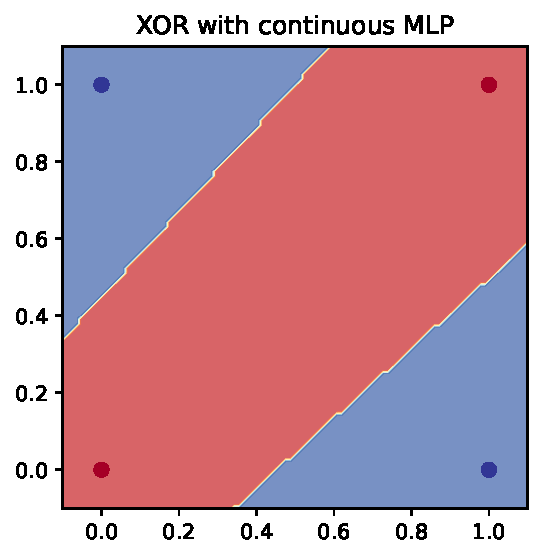
\includegraphics[scale=0.5]{../computational\_graphs/code/continuous_xor.pdf}
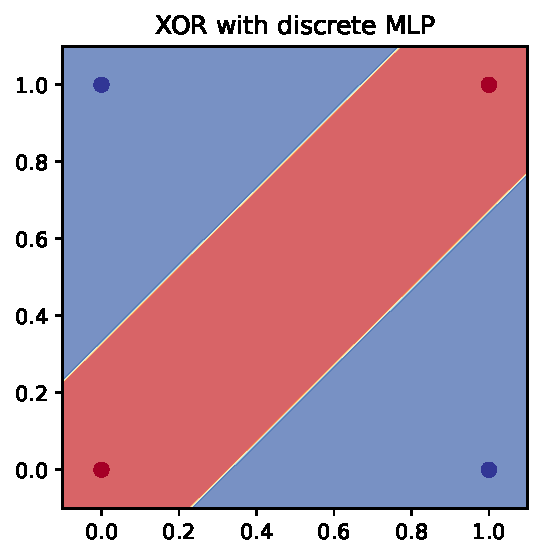
\includegraphics[scale=0.5]{../computational\_graphs/code/discrete_xor.pdf}

\caption{An example of quantization on a small neural network trained to compute xor. The network contains a unique hidden layer with 5 features.}

\end{figure}

\end{frame}

\section{Future work}
\begin{frame}{Instanciation of the Theory}

We pass a first sanity check: we can model a neural network with a generalized computation graph using near-semiring. We can discuss other possible instanciation:

\begin{itemize}

	\item Is layer-wise relevance propagation captured by the model?
	
	\item Is the work done by Antoine an instance of the model?
	
	\item Does the model allow to retrieve efficiently shapley values?
	
	\item Can the model be a theoretical basis for high-level circuits that explain neural networks, considering the near-semiring over the monoid $\Sigma^*$?

\end{itemize}


% Sanity check : we can model a NN. Do we generalize LRP ? Can we find Shapley values ? Can we use Shapley values to define the functions ?

% Application avec le monoïde $\Sigma ^ *$ : les fonctions linéraires sont la concaténation d'un mot (par exemple une arrête qui représente "est-ce qu'il y a un arc de cercle en haut à gauche de l'image" sera represente par l'arrete "_arc_cercle_hg_" et les activations non linéaires sont des sélections : la présence de "_arc_cercle_hg_", "_arc_cercle_hd_", "..._bg_" et "..._bd_" conduit à transformer le mot en "cercle" sinon on le transforme en le mot vide, par exemple.) Une telle généralité utilise toute la puissance de la théorie : aucun axiome n'est de trop, et on ne peut pas en rajouter (0 absorbant que d'un côté, pas de distributivité, pas de commu de \circ)

\end{frame}

\begin{frame}{Further Theoretical Development}

\begin{itemize}
	
	\item Investigate the differences between forward and backward modes.

	\item Investigate a potential theory of computation graphs with an algebraic derivation.

	\item Develop an analogous model for a coarse-grained provenance.

\end{itemize}

\end{frame}

\section{References}
\begin{frame}{References}

\bibliographystyle{apalike}
\bibliography{presentation_09_07.bib}

\end{frame}

\begin{frame}{Computer Science Universal Object for Near-semirings}

I lack a formal framework for retrieving a function from a graph.

\begin{block}{Theorem - Freely Generated Near-Semirings Capture Provenance}

	Given a computation graphs with $n$ edges, the 
	
\end{block}

\end{frame}

\section{Failed attempt - Differential Geometry}

\begin{frame}



\end{frame}

\cite{ramusat_semiring-based_2022}


\end{document}